
\begin{frame}[fragile]{QCheck}
    
Vérification de propriétés

\begin{figure}
    \centering
    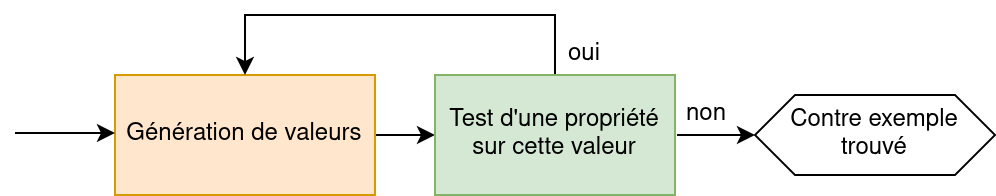
\includegraphics[width=0.9\textwidth]{slides/images/qcheck.drawio.png}
\end{figure}

\subtt{QCheck cherche un contre exemple minimal}

\begin{lstlisting}
type 'a generator
val small_int : int generator
val small_list : 'a generator -> 'a list generator
val Test.make : 'a generator -> ('a -> bool) -> Test.t
\end{lstlisting}

Plus d'informations: \url{https://github.com/c-cube/qcheck}
\end{frame}

\begin{frame}[fragile]{Exemple de test}

\begin{lstlisting}
let generateur = QCheck.(small_list small_int)
\end{lstlisting}

\subtt{Exemple 1 : }
\begin{lstlisting}
    (* forall l, List.rev (List.rev l) = l *)
    Test.make generateur 
        (fun l ->  List.rev (List.rev l) = l)
\end{lstlisting}
\pause
\subtt{Exemple 2 : }
\begin{lstlisting}
    (* forall l, int list, tri_fusion l est trié *)
    Test.make generateur
        (fun l ->  List.sort compare entree = tri_fusion entree)
\end{lstlisting}

\end{frame}

\begin{frame}[fragile]{Réduction}
    
\begin{lstlisting}
  let rev lst = 
    if List.length lst >= 5 then lst
    else List.rev lst
\end{lstlisting}
\subtt{Réduction du contre exemple}
\begin{lstlisting}
0   => [3176607639030078719; -702777917135807191; 1243225506173352439; -168141035741141589; 4478591693389419378; -2908482084465810011; -4471604993596125836; 2097048314685490782; -777119667999583759]
1   => [1243225506173352439; -168141035741141589; 4478591693389419378; -2908482084465810011; -4471604993596125836; 2097048314685490782; -777119667999583759]
200 => [0; 0; 0; 4095797489620100; -777119667999583759]
255 => [0; 0; 0; 0; -194279916999895940]
299 => [0; 0; 0; 0; -11044]
313 => [0; 0; 0; 0; -1]
\end{lstlisting}

\end{frame}

\begin{frame}{Simulation d'un état}

\begin{figure}
\centering
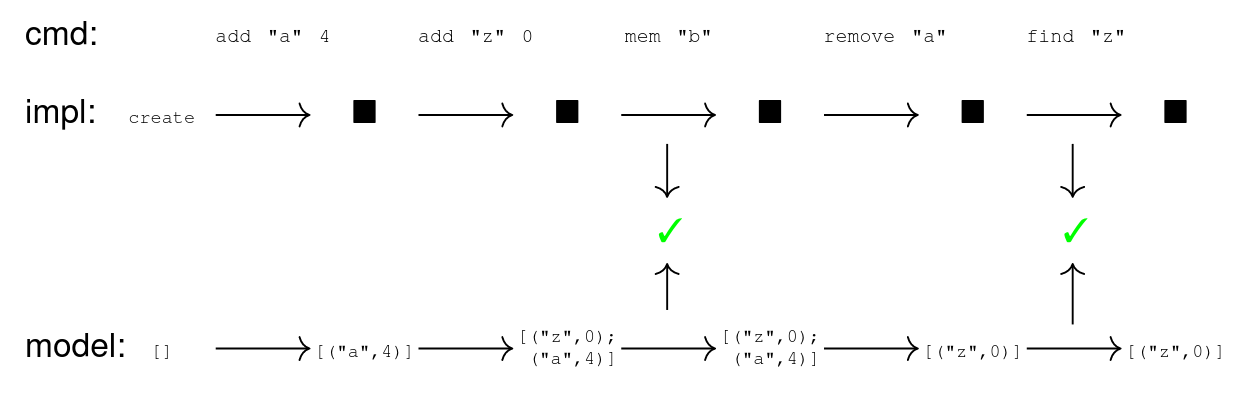
\includegraphics[width=\textwidth]{slides/images/qcheck_state.png}
\end{figure}
\begin{figure}
\centering
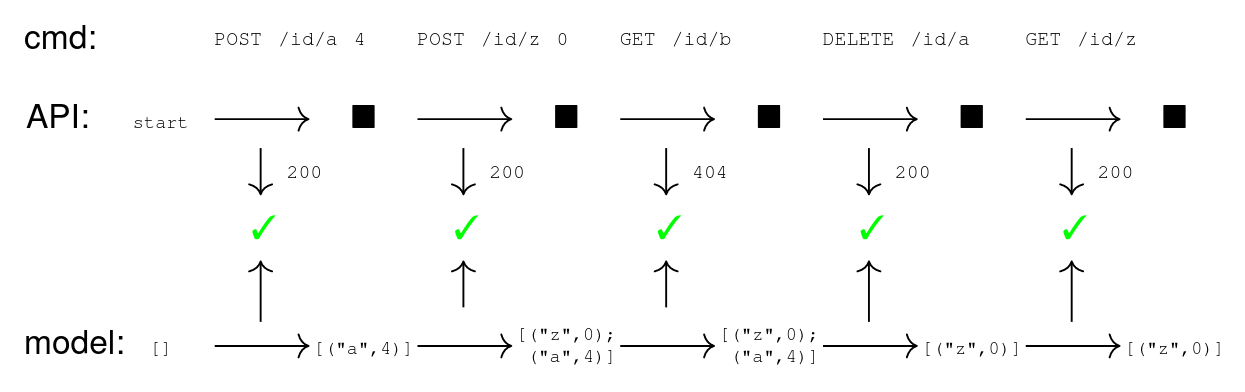
\includegraphics[width=\textwidth]{slides/images/qcheck_state_2.png}
\end{figure}

\end{frame}